\NeedsTeXFormat{LaTeX2e}
\documentclass[twocolumn,letterpaper]{igs}
%\documentclass[review,letterpaper]{igs}

\usepackage{stfloats}
\usepackage{verbatim,xspace,amsmath,amssymb,bm}

\usepackage{tikz}
\usetikzlibrary{arrows}

\usepackage{igsnatbib}  % see igs2eguide.tex for example citation styles

\newcommand{\onecol}[1]{\includegraphics[width=86mm]{#1}}
\newcommand{\twocol}[1]{\includegraphics[width=178mm]{#1}}

% math macros
\newcommand\bb{\mathbf{b}}
\newcommand\bc{\mathbf{c}}
\newcommand\bbf{\mathbf{f}}
\newcommand\bn{\mathbf{n}}
\newcommand\bq{\mathbf{q}}
\newcommand\bu{\mathbf{u}}
\newcommand\bv{\mathbf{v}}
\newcommand\by{\mathbf{y}}

\newcommand\bF{\mathbf{F}}
\newcommand\bH{\mathbf{H}}
\newcommand\bQ{\mathbf{Q}}
\newcommand\bV{\mathbf{V}}
\newcommand\bW{\mathbf{W}}
\newcommand\bX{\mathbf{X}}

\newcommand\CC{\mathbb{C}}
\newcommand{\DDt}[1]{\ensuremath{\frac{d #1}{d t}}}
\newcommand{\ddt}[1]{\ensuremath{\frac{\partial #1}{\partial t}}}
\newcommand{\ddx}[1]{\ensuremath{\frac{\partial #1}{\partial x}}}
\newcommand{\ddy}[1]{\ensuremath{\frac{\partial #1}{\partial y}}}
\newcommand{\ddxp}[1]{\ensuremath{\frac{\partial #1}{\partial x'}}}
\newcommand{\ddz}[1]{\ensuremath{\frac{\partial #1}{\partial z}}}
\newcommand{\ddxx}[1]{\ensuremath{\frac{\partial^2 #1}{\partial x^2}}}
\newcommand{\ddyy}[1]{\ensuremath{\frac{\partial^2 #1}{\partial y^2}}}
\newcommand{\ddxy}[1]{\ensuremath{\frac{\partial^2 #1}{\partial x \partial y}}}
\newcommand{\ddzz}[1]{\ensuremath{\frac{\partial^2 #1}{\partial z^2}}}
\newcommand{\Div}{\nabla\cdot}
\newcommand\eps{\epsilon}
\newcommand{\grad}{\nabla}
\newcommand{\ihat}{\mathbf{i}}
\newcommand{\ip}[2]{\ensuremath{\left<#1,#2\right>}}
\newcommand{\jhat}{\mathbf{j}}
\newcommand{\khat}{\mathbf{k}}
\newcommand{\nhat}{\mathbf{n}}
\newcommand\lam{\lambda}
\newcommand\lap{\triangle}
\newcommand\RR{\mathbb{R}}
\newcommand\vf{\varphi}

\newcommand{\Mstar}{$\text{M}^{\bigstar}$\xspace}
\newcommand{\Mstarnoup}{$\text{M}^{\bigstar}_{\text{no}}$\xspace}
\newcommand{\Mstarfullup}{$\text{M}^{\bigstar}_{\text{full}}$\xspace}

\newcommand\alpharight{\alpha_{{}_{\blacktriangleright}}}
\newcommand\alphaup{\alpha_{{\!}_{\blacktriangle}}}

\newcommand{\dxtwo}{\tfrac{\Delta x}{2}}
\newcommand{\dytwo}{\tfrac{\Delta y}{2}}

\newcommand{\half}{\tfrac{1}{2}}


\begin{document}

\title[Stable FVE schemes for the shallow ice approximation]{Stable finite volume element schemes \\ for the shallow ice approximation}

\abstract{The isothermal, non-sliding shallow ice approximation, combined with mass conservation, is a model for ice sheet and glacier flow which determines the ice geometry by the solution of a free-boundary problem.  We demonstrate a fully-implicit scheme with no stability restrictions by solving the steady state form of this problem directly, without time-stepping.  We first re-interpret \cite{Mahaffy1976} finite difference calculation as a ``finite volume element'' (FVE) scheme so that everywhere-defined numerical fields and a flux integral form of the conservation statement are both available in the construction of numerical schemes.  On this FVE basis we build an improved scheme which has both better quadrature in the integral and upwinding on that part of the flux which is proportional to the bed gradient.  The discrete equations are then solved by a parallel Newton scheme which respects the constraint that thicknesses are nonnegative.  The results show superior accuracy to any published results for both a flat bed and a bedrock-step \citep{JaroschSchoofAnslow2013} exact solution.  We then apply the improved scheme at 1km resolution to the compute the steady-state geometry of the Greenland ice sheet, using only bedrock elevation and present-day surface mass balance as input data, in a laptop-scale computation.}

\author{Ed Bueler}

\affiliation{Department of Mathematics and Statistics, and Geophysical Institute, University of Alaska Fairbanks, USA \\
E-mail: \emph{\texttt{elbueler\@@alaska.edu}}}

\maketitle

\sectionsize


\section*{Introduction}

The first successful numerical approach to modeling ice sheet flow and geometry evolution in two horizontal dimensions was the finite difference (FD) scheme introduced by \cite{Mahaffy1976}.  This scheme numerically solves the shallow ice approximation (SIA; Hutter, 1983)\nocite{Hutter1983} by computing the ice flux at staggered-grid points, using particular choices when evaluating the ice thickness and surface slope.  An advantage of the scheme is its relatively-small stencil, which reduces memory usage in implicit or semi-implicit implementations \citep{HindmarshPayne1996}.  The small stencil also reduces interprocess communication in parallel implementations \citep{Bueleretal2007}.  The stability and accuracy properties of the Mahaffy scheme, at least in an explicit time-stepping context, are relatively-well understood in flat-bed cases \citep{Bueleretal2005,HindmarshPayne1996}.

Most existing numerical models solve the time-dependent SIA with explicit or semi-implicit time-stepping  \citep{Bueleretal2005,EgholmNielsen2010,HindmarshPayne1996,Huybrechtsetal1996,JaroschSchoofAnslow2013}.  The time-stepping restrictions which arise in that context are needed partly to avoid classical instabilities at wavelengths comparable to the grid spacing \citep{MortonMayers2005}.  However, \cite{Bueleretal2005} and \cite{JaroschSchoofAnslow2013} point out that these schemes also involve \emph{ad hoc} treatment of the free margin of the ice sheet, for example using projection to reset computed negative thicknesses back to zero.  It would be desirable to escape both time-stepping restrictions and \emph{ad hoc} margin treatments by implicitly solving the SIA free boundary problem in a mathematically-principled manner.

% guess:
Earlier work on the free-boundary problem in one horizontal dimension \citep{Hindmarshetal1987,HindmarshHutter1988} avoided \emph{ad hoc} margin treatment by tracking the margin as a moving grid point.  Such margin-tracking does not easily extend to two dimensions, however, because the ice margin of real ice sheets is (essentially) a fractal curve, or at least a curve of minimal smoothness and variable topology.

Calvo and others (2000; 2002)\nocite{CalvoDuranyVazquez2000,Calvoetal2002} avoid \emph{ad hoc} margin treatment by describing the time-dependent problem as a parabolic complementarity problem which includes the constraint that ice thickness is never negative, but their work is limited to one horizontal dimension and flat beds only.  They solve each time step numerically by a projected Gauss-Siedel scheme \citep{Ciarlet2002}, which does not scale to large problems.  

\cite{JouvetBueler2012} pose and numerically-solve the steady state free boundary problem as a variational inequality \citep{KinderlehrerStampacchia1980}, based on the constraint of non-negative thickness, in two spatial dimensions and with nontrivial bed topography.  In this context the SIA model is a variational inequality which is not equivalent to a minimization problem, at least in the general non-flat-bed case.  \cite{JouvetBueler2012} therefore solve the full SIA equations by successive well-posed, but only approximate, minimization problems which converge to the full equations in a fixed-point iteration limit.  The success of this model is demonstrated by a 5 km grid steady-state calculation for Greenland using a piecewise-linear triangulation finite element (FE) method \citep{Elmanetal2005}.

\cite{JouvetGraeser2013} also solve the SIA component of their hybrid through a sequence of minimization problems.  These minimization problems arise from a time-splitting in which the objective functional is constructed partly by fixing the thickness from the previous time-step.  Each minimization problem is solved by a constraint-adapted form of the Newton iteration, ``TNNMG'', which includes a nonlinear multigrid resolution of the discrete equations.

We follow the \cite{JouvetBueler2012} approach of solving the steady state free boundary problem, but using a Mahaffy-like scheme on a structured rectangular mesh.  Furthermore after preliminary steps to generate a good first iterate, we apply the Newton iteration directly to the SIA free boundary problem, and not to a minimization approximation.  Specifically, we use a continuation scheme to generate an iterate in the domain of convergence of the Newton method, but the algorithm ends by showing quadratic convergence to the solution of the full SIA problem, which is not, as noted, a minimization problem.

The first part of the paper has a historical side, because we reinterpret the classical Mahaffy scheme as a finite-volume \citep[FV;][]{LeVeque2002} scheme which merely uses a non-standard quadrature choice in the conservation-of-mass flux integral.  But in this reinterpretation the integrand, the vertically-integrated ice flux, is defined everywhere because the ice thickness field lives in a continuous space of trial functions, unlike in the FD derivation of the scheme.  These trial functions are piecewise-bilinear on a structured grid of rectangles, that is, they are $Q^1$ finite elements \citep{Elmanetal2005}.  Thus our re-interpretation has both FV and FE aspects.  If we think of the method as a ``true'' FE method then the test functions must be piecewise-constant with support on dual rectangular control volumes, making a Petrov-Galerkin FE method \citep{Elmanetal2005}.  But it is more natural to regard the scheme as a ``finite volume element'' \citep[FVE;][]{Cai1990,EwingLinLin2002} method because the weak form, used in constructing fully-discrete schemes, is simply the flux integral itself, over control volumes, just as would appear in FV schemes.  We adopt the FVE terminology because we want the best of both worlds: the unknown thickness is defined everywhere (i.e.~FE trial functions) and the mass conservation equation is transparently stated in classical flux-integral form over control volumes (i.e.~as in an FV method).

Because we also successfully solve the whole free-boundary problem at once by a parallel Newton method, our improved scheme is shown to be unconditionally stable as a fully-implicit scheme.  Our parallel implementation of the scheme uses Newton solvers adapted to inequality constraints \citep{BensonMunson2006} which are included in the open-source PETSc library \citep{Balayetal2014}.

Our paper is organized as follows.  We start with a statement of the steady, isothermal SIA model.  We then recall the classical Mahaffy scheme in FD form before re-interpreting it as an FVE scheme and identifying its non-standard midpoint rule application in the flux integral.  Building off this re-interpretation we identify better quadrature in the flux integral, and we then add a bit of first-order upwinding on the part of the flux that comes from the bedrock slope.  The resulting improved scheme, which has the same stencil as the classical Mahaffy scheme, is called ``\Mstar.''  Next we describe the Newton solver which we apply to the discrete equations and constraints.  Results are then given in verification cases.  They are at least as good as those from higher-resolution upwind schemes when applied to the \cite{JaroschSchoofAnslow2013} bedrock-step exact solution.  Then we show how the method is applied to real ice sheets by computing, without time-stepping but at very 1 km high resolution, the steady state shape of the Greenland ice sheet in a present-day modeled climate.

In the Appendix A we describe how to construct, on certain unstructured finite element triangulations, an analog of the \Mstar scheme.  Appendix B addresses the analytical calculation of the Jacobian in the \Mstar scheme.


\section*{The continuum model}

The time-dependent evolution equation for the ice thickness $H$ is mass conservation:
\begin{equation}
\frac{\partial H}{\partial t} + \Div \bq = m.  \label{eq:siaevolution}
\end{equation}
Here $\bq$ denotes the vertically-integrated flux and $m$ is the surface mass balance, also called the accumulation/ablation function.  The thickness $H$ cannot be determined merely by mass conservation, however, and a relation between $H$ and $\bq$ is needed.

The shallow ice approximation (SIA) is the simplest such model in common use in glaciology.  It is the lubrication approximation \citep{Fowler1997} of the Stokes equations for slow-flowing ice, in non-sliding contact with the bed.  We only consider the isothermal, Glen-power-law \citep{GreveBlatter2009} case.  Let $b$ be the bed and $s = H+b$ the ice surface elevation.  The flux $\bq$ is given by
\begin{equation}
\bq = - \Gamma H^{n+2} |\grad s|^{n-1} \grad s  \label{eq:siaflux}
\end{equation}
where $\Gamma = 2 A (\rho g)^n / (n+2)$ is a positive constant derived from the power $n\ge 1$, ice softness $A$, ice density $\rho$, and gravity $g$.

The flux $\bq$ has multiple functional forms which are equivalent to \eqref{eq:siaflux}.  Because equations \eqref{eq:siaevolution} and \eqref{eq:siaflux} are often interpreted as a single nonlinear diffusion equation \citep{Huybrechtsetal1996}, it is common to write
\begin{equation}
\bq = - D \grad s \quad \text{and} \quad D =  \Gamma H^{n+2} |\grad s|^{n-1}. \label{eq:siafluxdiffusion}
\end{equation}
However, if the bed is not flat then $\grad s$ and $\grad H$ are different and so the flux is not strictly diffusive (i.e.~where the flux is opposite to the gradient of the conserved quantity).  On the other hand one can compute a vertically-averaged velocity $\bV$, and then treat the flux as arising from the transport of the thickness by $\bV$, that is,
\begin{equation}
\bq = \bV H \quad \text{where} \quad \bV = - \Gamma H^{n+1} |\grad s|^{n-1} \grad s. \label{eq:siafluxvelocity}
\end{equation}
In this case \eqref{eq:siaevolution} is apparently a hyperbolic conservation equation, but this appearance is deceiving because the velocity depends in part on the gradient of the transported quantity.

The diffusion interpretation \eqref{eq:siafluxdiffusion} is appropriate in the flat-bed case because \eqref{eq:siaevolution} and \eqref{eq:siaflux} can then be transformed to a $p$-Laplacian diffusion equation \citep{Calvoetal2002}.  In general, however, the diffusion-equation interpretation is obscured by a nonzero bed gradient $\grad b$.  It is a barrier to theoretical progress on proving the existence and uniqueness of solutions \citep{JouvetBueler2012} and it generates conservation errors at the ice margin in numerical schemes \citep{JaroschSchoofAnslow2013}.  In fact, \cite{JaroschSchoofAnslow2013} propose a third form for the flux, namely
\begin{equation}
   \bq = \boldsymbol{\omega} H^{n+2} \quad \text{where} \quad \boldsymbol{\omega} = - \Gamma |\grad s|^{n-1} \grad s. \label{eq:siafluxjsa}
\end{equation}
The vector field $\boldsymbol{\omega}$ can be thought of as a ``velocity'' which transports $H^{n+2}$, and in this thinking the combination of \eqref{eq:siaevolution} and \eqref{eq:siafluxjsa} becomes a kind of nonlinear hyperbolic equation, but again with a ``velocity'' $\boldsymbol{\omega}$ that actually depends on the gradient of the transported quantity $H$.

We modify forms \eqref{eq:siafluxdiffusion} and \eqref{eq:siafluxjsa} to a split form
\begin{equation}
\bq = - D \grad H + \bW H^{n+2},\label{eq:fluxform}
\end{equation}
where $D$ is the same as in \eqref{eq:siafluxdiffusion} and where
\begin{equation}
\bW = - \Gamma |\grad s|^{n-1} \grad b.  \label{eq:siaWdefine}
\end{equation}
The vector field $\bW$ again transports $H^{n+2}$, but in this case it is proportional to $\grad b$ so only its magnitude is related to $\grad H$.  Note that $\bW=0$ in the case of flat beds, while $\boldsymbol{\omega}$ is both nonzero and diffusive in that case.

The combination of \eqref{eq:siaevolution} with any of the above forms for the flux $\bq$ defines a highly-nonlinear diffusion-advection equation.  In numerical schemes form \eqref{eq:fluxform} has the advantage that we can apply a non-oscillatory transport scheme to the ``$\bW H^{n+2}$'' term while also preserving accuracy by applying a centered scheme to the diffusive term ``$-D \grad H$''.  The presence of the often-dominant leading-order diffusion is also a motivation to use implicit time-stepping.  However, implicit schemes for \eqref{eq:siaevolution} also need to determine the location of the free boundary at each time step.

In this paper we will only solve the steady-state form of \eqref{eq:siaevolution}, namely
\begin{equation}
\Div \bq = m.  \label{eq:siasteady}
\end{equation}
Equivalently, by the divergence theorem applied to any subregion $V$ of $\Omega$ we get the flux-integral form of the steady-state SIA,
\begin{equation}
  \int_{\partial V} \bq \cdot \bn\,ds = \int_V m\, dx\,dy. \label{eq:siaasconservation}
\end{equation}
Here $\partial V$ denotes the boundary of $V$, $\bn$ is the outward normal unit vector, and $ds$ is the length element on the closed curve $\partial V$.

Equation \eqref{eq:siasteady}, or \eqref{eq:siaasconservation}, is a boundary-value problem in which the location where the boundary conditions should be applied is unknown \citep{JaroschSchoofAnslow2013,JouvetBueler2012}.  The ice-covered domain where \eqref{eq:siasteady} applies, and the location of the boundary where $H=0$ and $\bq=0$, cannot be treated as a small modification of a known boundary, though that is the standard approach of explicit time-stepping schemes for equation \eqref{eq:siaevolution} \citep{Bueleretal2005,Huybrechtsetal1996}.

To be more precise about boundary conditions, if the surface mass balance $m$ is sufficiently-negative near the boundary of the domain $\Omega$ on which \eqref{eq:siasteady} is intended to be solved then $H\to 0$ at points inside $\Omega$.  These points define the free boundary, at which $\bq \to 0$ simultaneously \citep{JouvetBueler2012}.  Because of the factor $H^{n+2}$ in formula \eqref{eq:siafluxdiffusion} for the diffusivity $D$, the problem also has degenerate diffusivity, i.e.~also $D \to 0$ at the free boundary.  Solving equation \eqref{eq:siasteady}, or computing a time-step of \eqref{eq:siaevolution}, as such a free-boundary problem, without a boundary flux applied along any part of the boundary of $\Omega$, is usually called a ``whole'' ice sheet model.  We restrict our attention to such whole ice sheet models.

The problem we solve combines equations \eqref{eq:fluxform} and \eqref{eq:siasteady}, where $D$ and $\bW$ are defined in \eqref{eq:siafluxdiffusion} and \eqref{eq:siaWdefine} respectively.  The input data consists of the bed elevation $b(x,y)$ and the (steady) surface mass balance $m(x,y)$.  Both of these input fields are defined on some larger domain $\Omega$ than the ice-covered set, and we assume $m$ sufficiently-negative near the boundary of $\Omega$ so that the ice-covered set is surrounded by a free boundary.  The solution is the nonnegative thickness function $H(x,y)$, defined everywhere in $\Omega$ but zero where there is no ice, and corresponding surface elevation $s(x,y)=H(x,y)+b(x,y)$.


\section{The classical Mahaffy scheme}   \label{sec:mahaffyfd}

Consider the rectangular structured FD grid, with spacing $\Delta x,\Delta y$, shown in Figure \ref{fig:fdfemgrids}a.  The \cite{Mahaffy1976} scheme calculates one flux component at each of the staggered grid points marked by triangles.  For these points we introduce notation
\begin{equation}
x_j^\pm = x_j \pm \dxtwo, \qquad y_k^\pm = y_k \pm \dytwo. \label{eq:definexypm}
\end{equation}
At $(x_j^+,y_k)$ the scheme computes the $x$-component of the flux by
\begin{equation}
q^x_{j+\half,k} = - \Gamma (\hat H_{j+\half,k})^{\,n+2} \alpharight^{\,n-1} \frac{s_{j+1,k} - s_{j,k}}{\Delta x}  \label{eq:mahaffyqx}
\end{equation}
where $s_{j,k} = H_{j,k} + b_{j,k}$,
\begin{equation}
  \hat H_{j+\half,k} = \frac{H_{j,k} + H_{j+1,k}}{2},  \label{eq:mahaffyHav}
\end{equation}
and ``$\alpharight$\!'' is an estimate of $|\grad s|$:
\begin{align}
\alpharight^{\,2} &= \left(\frac{s_{j+1,k} - s_{j,k}}{\Delta x}\right)^2  \label{eq:mahaffyalphax} \\
  &\quad + \left(\frac{s_{j,k+1} + s_{j+1,k+1} - s_{j,k-1} - s_{j+1,k-1}}{4 \Delta y}\right)^2. \notag
\end{align}
At $(x_j,y_k^+)$ the scheme computes
\begin{equation}
q^y_{j,k+\half} = - \Gamma (\hat H_{j,k+\half})^{\,n+2} \alphaup^{\,n-1} \frac{s_{j,k+1} - s_{j,k}}{\Delta y}  \label{eq:mahaffyqy}
\end{equation}
where $\hat H_{j,k+\half}$ and $\alphaup$ are defined by swapping the roles of $j$ and $k$, and $\Delta x$ and $\Delta y$, in equations \eqref{eq:mahaffyHav} and \eqref{eq:mahaffyalphax}, respectively.  The slope approximation in \eqref{eq:mahaffyalphax}, and the corresponding formula for $\alphaup$, is perhaps the least-obvious aspect of the Mahaffy scheme, but it is easy to check that these FD formulas are consistent \citep{MortonMayers2005}.

\begin{figure}[ht]
\begin{center}
\begin{tikzpicture}[scale=0.75]
  %uncomment to see grid on which it was generated:
  %\draw[dotted,step=1.0,black,very thin] (0,0) grid (6,4);

  % faint grid
  \draw[gray, dashed] (-0.75,0) -- (6.75,0);
  \draw[gray, dashed] (-0.75,2) -- (6.75,2);
  \draw[gray, dashed] (-0.75,4) -- (6.75,4);
  \draw[gray, dashed] (0,-0.5) -- (0,4.5);
  \draw[gray, dashed] (3,-0.5) -- (3,4.5);
  \draw[gray, dashed] (6,-0.5) -- (6,4.5);

  % regular FD points
  \filldraw (0,0) circle (2.5pt);
  \filldraw (3,0) circle (2.5pt);
  \filldraw (6,0) circle (2.5pt);
  \filldraw (0,2) circle (2.5pt);
  \filldraw (3,2) circle (2.5pt);
  \filldraw (6,2) circle (2.5pt);
  \filldraw (0,4) circle (2.5pt);
  \filldraw (3,4) circle (2.5pt);
  \filldraw (6,4) circle (2.5pt);

  % staggered FD points
  \def\dx{0.12};
  \filldraw (1.5-\dx,2+\dx) -- (1.5+\dx,2) -- (1.5-\dx,2-\dx) -- cycle;
  \filldraw (4.5-\dx,2+\dx) -- (4.5+\dx,2) -- (4.5-\dx,2-\dx) -- cycle;
  \filldraw (3-\dx,1-\dx) -- (3,1+\dx) -- (3+\dx,1-\dx) -- cycle;
  \filldraw (3-\dx,3-\dx) -- (3,3+\dx) -- (3+\dx,3-\dx) -- cycle;

  % dimensions \Delta x, \Delta y
  \draw[latex-latex] (3.2,4.5) -- (5.8,4.5);
  \draw (4.5,5.0) node {$\Delta x$};
  \draw[latex-latex] (6.5,2.2) -- (6.5,3.8);
  \draw (7.0,3) node {$\Delta y$};

  % label center point and dims
  \draw (3,-1.0) node {$x_j$};
  \draw (-1.25,2) node {$y_k$};

  % label as "a"
  \draw (-1.5,5.5) node {{\large a.}};
\end{tikzpicture}
 \quad 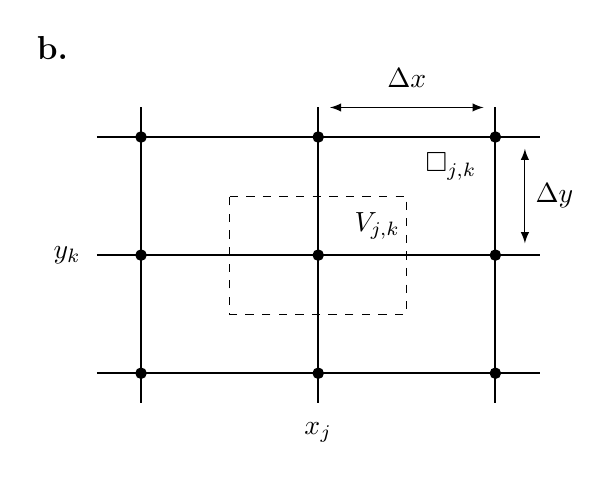
\begin{tikzpicture}[scale=0.75]
  %uncomment to see grid on which it was generated:
  %\draw[dotted,step=1.0,black,very thin] (0,0) grid (6,4);

  % strong grid around elements
  \draw[thick] (-0.75,0) -- (6.75,0);
  \draw[thick] (-0.75,2) -- (6.75,2);
  \draw[thick] (-0.75,4) -- (6.75,4);
  \draw[thick] (0,-0.5) -- (0,4.5);
  \draw[thick] (3,-0.5) -- (3,4.5);
  \draw[thick] (6,-0.5) -- (6,4.5);

  % nodes
  \filldraw (0,0) circle (2.5pt);
  \filldraw (3,0) circle (2.5pt);
  \filldraw (6,0) circle (2.5pt);
  \filldraw (0,2) circle (2.5pt);
  \filldraw (3,2) circle (2.5pt);
  \filldraw (6,2) circle (2.5pt);
  \filldraw (0,4) circle (2.5pt);
  \filldraw (3,4) circle (2.5pt);
  \filldraw (6,4) circle (2.5pt);

  % outline control volume
  \draw[dashed] (1.5,3) -- (4.5,3) -- (4.5,1) -- (1.5,1) -- cycle;

  % label element and control volume
  \draw (5.25,3.5) node {$\square_{j,k}$};
  \draw (4,2.5) node {$V_{j,k}$};

  % dimensions \Delta x, \Delta y
  \draw[latex-latex] (3.2,4.5) -- (5.8,4.5);
  \draw (4.5,5.0) node {$\Delta x$};
  \draw[latex-latex] (6.5,2.2) -- (6.5,3.8);
  \draw (7.0,3) node {$\Delta y$};

  % label center point and dims
  \draw (3,-1.0) node {$x_j$};
  \draw (-1.25,2) node {$y_k$};

  % label as "b"
  \tikzstyle{fontbf} = [font=\bf]
  \draw (-1.5,5.5) node[fontbf] {{\large b.}};
\end{tikzpicture}

\end{center}
\caption{\textbf{a.}~A structured FD grid with regular points (dots) and staggered points (triangles).  \textbf{b.}~The same grid as an FVE grid with rectangular elements $\square_{j,k}$ (solid), nodes (dots), a dual rectangular control volume $V_{j,k}$ (dashed), and Mahaffy-scheme flux-evaluation locations (circles).  Corners $\ell=0,1,2,3$ of the element are where each basis function $\chi_\ell$ equals one.}
\label{fig:fdfemgrids}
\end{figure}

The discretization of mass conservation equation \eqref{eq:siasteady} itself is straightforward.  In the steady case the scheme uses centered-differences \citep{MortonMayers2005}:
\begin{equation}
\frac{q^x_{j+1/2,k} - q^x_{j-1/2,k}}{\Delta x} + \frac{q^y_{j,k+1/2}- q^y_{j,k-1/2}}{\Delta y} = m_{j,k}.  \label{eq:siasteadyfd}
\end{equation}

Equation \eqref{eq:siasteadyfd}, combined with equations \eqref{eq:mahaffyqx} and \eqref{eq:mahaffyqy}, gives one equation in an algebraic system which determines all values $H_{j,k}$ simultaneously.  Equation \eqref{eq:siasteadyfd} relates the nine unknown values of $H$ at the regular grid points in Figure \ref{fig:fdfemgrids}a, the ``stencil''  \citep{MortonMayers2005} of the scheme.


\section{An FVE re-interpretation} \label{sec:fveinterpretation}

The above description of the Mahaffy FD method is familiar to numerical ice sheet modelers, but we now re-derive the scheme from an FE \emph{and} FV perspective.  As Figure \ref{fig:fdfemgrids} suggests, our re-interpretation uses the same structured grid, but the regular grid points are now nodes (degrees of freedom) for a continuous space of trial functions.  In fact, an FVE method supposes that the approximation $H^h$ of the solution lies in a finite-dimensional space of continuous functions which are sufficiently well-behaved so that the approximate flux $\bq^h$ is defined almost everywhere and can be integrated along $\partial V$ in \eqref{eq:siaasconservation}.  However, as in an FV method, integral equation \eqref{eq:siaasconservation} is only required to hold for a finite set of node-centered control volumes $V$ which together tile $\Omega$.  This generates a finite system of nonlinear algebraic equations.

In Figure \ref{fig:fdfemgrids}b, element $\square_{j,k}$ is the rectangle with lower-left corner at $(x_j,y_k)$.  When associated with bilinear functions this rectangle is a $Q^1$ finite element \citep{Elmanetal2005}.  A basis for bilinear functions on $\square_{j,k}$ is the set
\begin{equation}
\chi_\ell \left(\frac{x-x_j}{\Delta x},\frac{y-y_k}{\Delta y}\right), \label{eq:elementbasis}
\end{equation}
for $\ell=0,1,2,3$, where
\begin{align*}
\chi_0(\xi,\eta) &= \left(1-\xi\right) \left(1-\eta\right), & \chi_1(\xi,\eta) &= \xi \left(1-\eta\right), \\
\chi_2(\xi,\eta) &= \xi \eta, & \chi_3(\xi,\eta) &= \left(1-\xi\right) \eta.
\end{align*}
With this order, $\chi_\ell=1$ on element corners traversed in counter-clockwise order (Figure \ref{fig:fdfemgrids}b).  

Let
\begin{equation}
S_h = \{u \text{ is bilinear on each $\square_{j,k}$}\}
\end{equation}
be the trial space.  Functions in $S_h$ have a gradient which is defined almost everywhere, but the gradient is discontinuous along the element edges (solid lines in Figure \ref{fig:fdfemgrids}b).  We seek an approximate solution $H^h$ from $S_h$.  Also let $b^h$ be the piecewise-bilinear interpolant of the bed elevation $b$, and let $s^h=H^h+b^h$, so both $b^h$ and $s^h$ are in $S_h$.  We denote by $\bq^h$ the flux computed from formula \eqref{eq:siaflux} or \eqref{eq:fluxform} using $H^h$ and $b^h$, so $\bq^h$ is well-defined on the interior of each element.

Let $V_{j,k}$ be the control volume with center at $(x_j,y_j)$ (Figure \ref{fig:fdfemgrids}b).  In the FVE method we require \eqref{eq:siaasconservation} to hold for $\bq=\bq^h$ and $V$ equal to each $V_{j,j}$.  We will use a periodic grid with $N_x$ rectangles in the $x$-direction and $N_y$ in the $y$ direction, so there are $N=N_xN_y$ distinct control volumes  and thus $N$ equations in the resulting algebraic system.

\begin{figure}[ht]
\begin{center}
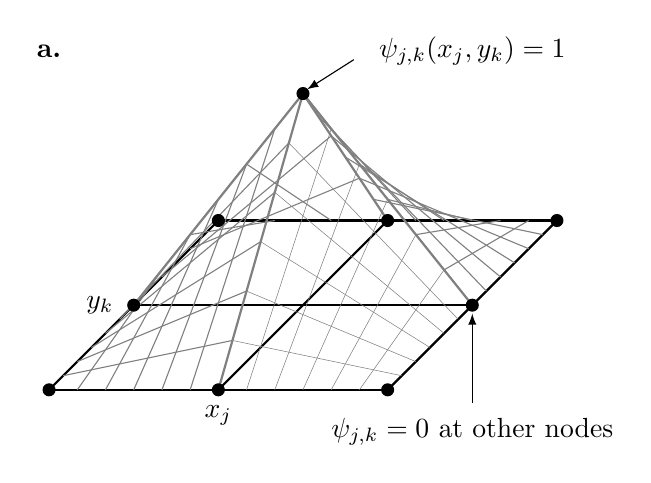
\begin{tikzpicture}[scale=8.6cm/16.0cm]
% min x = 0, max x = 12  so  width = 12 cm, but we pad
% 8.6cm is one-column width for J Glaciol
%\begin{tikzpicture}[scale=0.5]

  % strong grid around elements
  \draw[thick] (0,0) -- (8,0);
  \draw[thick] (2,2) -- (10,2);
  \draw[thick] (4,4) -- (12,4);
  \draw[thick] (0,0) -- (4,4);
  \draw[thick] (4,0) -- (8,4);
  \draw[thick] (8,0) -- (12,4);

  \def\ytop{7};

  % tent lines
  \draw[gray,thick] (6,\ytop) -- (4,0);
  \draw[gray,thick] (6,\ytop) -- (2,2);
  \draw[gray,thick] (6,\ytop) -- (10,2);
  \draw[gray,thick] (6,\ytop) -- (8,4);

  \def\dx{(10.0-6.0)/6};
  \def\dy{(2.0-\ytop)/6};
  \foreach \jj in {1,...,5}
  {
       \draw[gray,very thin] ({6+\jj*\dx},{\ytop+\jj*\dy}) -- ({4+(4/6)*\jj},0.0);
  }

  \def\dx{(4.0-6.0)/6};
  \def\dy{(0.0-\ytop)/6};
  \foreach \jj in {1,...,5}
  {
       \draw[gray,very thin] ({6+\jj*\dx},{\ytop+\jj*\dy}) -- ({10-(2/6)*\jj},{2-(2/6)*\jj});
  }

  \def\dx{(2.0-6.0)/6};
  \def\dy{(2.0-\ytop)/6};
  \foreach \jj in {1,...,5}
  {
       \draw[gray,thin] ({6+\jj*\dx},{\ytop+\jj*\dy}) -- ({4-(4/6)*\jj},0.0);
  }

  \def\dx{(4.0-6.0)/6};
  \def\dy{(0.0-\ytop)/6};
  \foreach \jj in {1,...,5}
  {
       \draw[gray,thin] ({6+\jj*\dx},{\ytop+\jj*\dy}) -- ({2-(2/6)*\jj},{2-(2/6)*\jj});
  }

  \def\dx{(10.0-6.0)/6};
  \def\dy{(2.0-\ytop)/6};
  \foreach \jj in {1,...,5}
  {
       \draw[gray,thin] ({6+\jj*\dx},{\ytop+\jj*\dy}) -- ({8+(4/6)*\jj},4.0);
  }

  \def\dx{(8.0-6.0)/6};
  \def\dy{(4.0-\ytop)/6};
  \foreach \jj in {1,...,5}
  {
       \draw[gray,thin] ({6+\jj*\dx},{\ytop+\jj*\dy}) -- ({10+(2/6)*\jj},{2+(2/6)*\jj});
  }

  \def\dx{(2.0-6.0)/3};
  \def\dy{(2.0-\ytop)/3};
  \foreach \jj in {1,...,2}  % reduce clutter
  {
       \draw[gray,thin] ({6+\jj*\dx},{\ytop+\jj*\dy}) -- ({8-(4/3)*\jj},4.0);
  }

  \def\dx{(8.0-6.0)/3};
  \def\dy{(4.0-\ytop)/3};
  \foreach \jj in {1,...,2}
  {
       \draw[gray,thin] ({6+\jj*\dx},{\ytop+\jj*\dy}) -- ({2+(2/3)*\jj},{2+(2/3)*\jj});
  }

  % nodes in base plane
  \filldraw (0,0) circle (4pt);
  \filldraw (4,0) circle (4pt);
  \filldraw (8,0) circle (4pt);
  \filldraw (2,2) circle (4pt);
  %\filldraw (6,2) circle (4pt);   % (x_j,y_k) is at (6,2)
  \filldraw (10,2) circle (4pt);
  \filldraw (4,4) circle (4pt);
  \filldraw (8,4) circle (4pt);
  \filldraw (12,4) circle (4pt);

  % node at tent top
  \filldraw (6,\ytop) circle (4pt);

  % annotate
  \draw (10,\ytop+1.0) node {$\psi_{j,k}(x_j,y_k)=1$};
  \draw[-latex] (7.2,\ytop+0.8) -- (6.1,\ytop+0.1);
  \draw (10,-1.0) node {$\psi_{j,k}=0$ at other nodes};
  \draw[-latex] (10,-0.3) -- (10,1.8);

  % label center point
  \draw (4,-0.6) node {$x_j$};
  \draw (1.2,2) node {$y_k$};

  % label as "a"
  \tikzstyle{fontbf} = [font=\bf]
  \draw (0,8) node[fontbf] {a.};

\end{tikzpicture}
 \quad 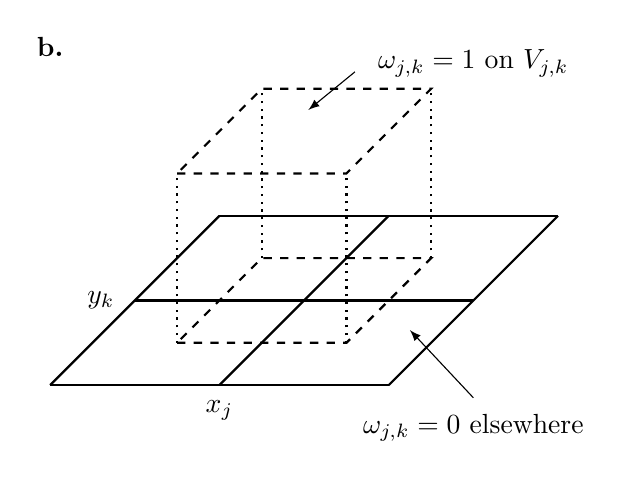
\begin{tikzpicture}[scale=8.6cm/16.0cm]
% min x = 0, max x = 12  so  width = 12 cm, but we pad
% 8.6cm is one-column width for J Glaciol
%\begin{tikzpicture}[scale=0.5]

  % strong grid around elements
  \draw[thick] (0,0) -- (8,0);
  \draw[thick] (2,2) -- (10,2);
  \draw[thick] (4,4) -- (12,4);
  \draw[thick] (0,0) -- (4,4);
  \draw[thick] (4,0) -- (8,4);
  \draw[thick] (8,0) -- (12,4);

  % dashed grid around control volume in base plane
  \draw[thick] (0,0) -- (8,0);

  % label element and control volume
  \def\lift{4};
  \draw[dashed, thick] (3,1) -- (7,1) -- (9,3) -- (5,3) -- cycle;
  \draw[dashed, thick] (3,1+\lift) -- (7,1+\lift) -- (9,3+\lift) -- (5,3+\lift) -- cycle;
  \draw[dotted, thick] (3,1) -- (3,1+\lift);
  \draw[dotted, thick] (7,1) -- (7,1+\lift);
  \draw[dotted, thick] (9,3) -- (9,3+\lift);
  \draw[dotted, thick] (5,3) -- (5,3+\lift);

  % annotate
  \draw (10,\lift+3.6) node {$\omega_{j,k}=1$ on $V_{j,k}$};
  \draw[-latex] (7.2,\lift+3.4) -- (6.1,\lift+2.5);
  \draw (10,-1.0) node {$\omega_{j,k}=0$ elsewhere};
  \draw[-latex] (10,-0.3) -- (8.5,1.3);

  % label center point
  \draw (4,-0.6) node {$x_j$};
  \draw (1.2,2) node {$y_k$};

  % label as "b"
  \tikzstyle{fontbf} = [font=\bf]
  \draw (0,8) node[fontbf] {b.};

\end{tikzpicture}

\end{center}
\caption{\textbf{a.}~A continuous ``hat'' basis function $\psi_{j,k}(x,y)$ in the trial space $S_h$.  \textbf{b.}~A discontinuous, piecewise-constant basis function $\omega_{j,k}(x,y)$ in the test space $S_h^*$.}
\label{fig:fembases}
\end{figure}

Instead of control volumes we could introduce test functions.  Let
\begin{equation}
S_h^* = \{u \text{ is constant on each $V_{j,k}$}\}
\end{equation}
be functions which are piecewise-constant and discontinuous only along the control volume edges (dashed lines in Figure \ref{fig:fdfemgrids}b).  Note that bases of $S_h$ and $S_h^*$ are formed by those functions which take value one at a single node, and zero at all other nodes.  We write $\psi_{j,k}(x,y)$ for the unique function in $S_h$ so that $\psi_{j,k}(x_r,y_s) = \delta_{jr} \delta_{ks}$, while $\omega_{j,k}(x,y)$ is the unique function in $S_h^*$ so that $\omega_{j,k}(x_r,y_s) = \delta_{jr} \delta_{ks}$; see Figure \ref{fig:fembases}.  Requiring \eqref{eq:siaasconservation} to hold for each control volume, as in the FVE method, is equivalent to multiplying \eqref{eq:siasteady} by $\omega_{j,k}$ and then integrating-by-parts.  Such a calculation requires the generalized-function idea that the derivative of a step function is a Dirac delta function.  From now on, however, we will use the FVE interpretation, and thus not need test functions or $S_h^*$.

Both the classical Mahaffy scheme, and our improved scheme below, assume midpoint quadrature on the right-hand integral in \eqref{eq:siaasconservation}.  Thus the FVE method is this: we seek $H^h$ in $S_h$ satisfying
\begin{equation}
  \int_{\partial V_{j,k}} \bq^h \cdot \bn\,ds = m_{j,k}\, \Delta x \Delta y, \label{eq:siafve}
\end{equation}
for all $j,k$.  It remains to choose a quadrature rule on the left, however.

We decompose the integral in \eqref{eq:siafve} into the four edges which form $\partial V_{j,k}$:
\begin{align}
\int_{\partial V_{j,k}} \bq^h \cdot \bn\,ds &= \int_{y_k^-}^{y_k^+} q^x(x_j^+,y)\,dy \label{eq:fluxintdecomp} \\
&\quad + \int_{x_j^-}^{x_j^+} q^y(x,y_k^+)\,dx \notag \\
&\quad - \int_{y_k^-}^{y_k^+} q^x(x_j^-,y)\,dy \notag \\
&\quad - \int_{x_j^-}^{x_j^+} q^y(x,y_k^-)\,dx. \notag
\end{align}
Though $\bq^h$ is a well-defined, bounded function, it is discontinuous across element boundaries.  For example, in the first integral on the right in \eqref{eq:fluxintdecomp} the integrand $f(y) = q^x(x_j^+,y)$ has a jump discontinuity at the midpoint $y=y_k$ of the interval of integration because $s^h_y$ is discontinuous there.  On the other hand, formula \eqref{eq:mahaffyqx} in the Mahaffy FD scheme computes the normal component of $\bq^h$ exactly at $y=y_k$.

The key to the Mahaffy scheme is that it computes each integral in \eqref{eq:fluxintdecomp} by the midpoint method, but by \emph{averaging the discontinuous component of the surface gradient across its jump discontinuity}.  Mahaffy does not use a true quadrature because the integrand $\bq^h\cdot \bn$ does not have a value at the quadrature point.

To turn this idea into formulas, observe that the thickness $H^h$ and the $x$-derivative $\partial s^h/\partial x = s^h_x$ are continuous along the edge between elements $\square_{j,k}$ and $\square_{j,k-1}$.  Indeed, using the element basis \eqref{eq:elementbasis} the surface gradient on $\square_{j,k}$ has components
\begin{align}
s^h_x(x,y) &= \frac{s_{j+1,k}-s_{j,k}}{\Delta x} \left(1-\frac{y-y_k}{\Delta y}\right)  \label{eq:grads} \\
   &\quad + \frac{s_{j+1,k+1}-s_{j,k+1}}{\Delta x} \left(\frac{y-y_k}{\Delta y}\right), \notag \\
s^h_y(x,y) &= \frac{s_{j,k+1}-s_{j,k}}{\Delta y} \left(1-\frac{x-x_j}{\Delta x}\right) \notag \\
   &\quad + \frac{s_{j+1,k+1}-s_{j+1,k}}{\Delta y} \left(\frac{x-x_j}{\Delta x}\right). \notag
\end{align}
The same functions on $\square_{j,k-1}$ can be calculated by shifting the index $k$ to $k-1$.  Thus the continuous function $s^h_x(x,y)$ has value
\begin{equation}
s^h_x(x_j^+,y_k) = \frac{s_{j+1,k}-s_{j,k}}{\Delta x} \label{eq:femsxstag}
\end{equation}
at the midpoint in the first integral in \eqref{eq:fluxintdecomp}.  Similarly, writing-out $H^h(x,y)$ using the element basis \eqref{eq:elementbasis} gives
\begin{equation}
H^h(x_j^+,y_k) = \frac{H_{j,k}+H_{j+1,k}}{2} \label{eq:femHstag}
\end{equation}
at the midpoint, which is \eqref{eq:mahaffyHav}.  But the $y$-derivative $\partial s^h/\partial y = s^h_y$ has different values above (on $\square_{j,k}$) and below (on $\square_{j,k-1}$) the element boundary at $y = y_k$; the limits are:
\begin{align}
s^h_y(x_j^+,y_k\!+\!0) = \frac{s_{j,k+1}-s_{j,k} + s_{j+1,k+1}-s_{j+1,k}}{2\Delta y}, \\
s^h_y(x_j^+,y_k\!-\!0) = \frac{s_{j,k}-s_{j,k-1} + s_{j+1,k}-s_{j+1,k-1}}{2\Delta y}. \notag
\end{align}
The average of these values is not a value of $s_y^h$, but a re-construction thereof:
\begin{equation}
\widehat{s^h_y}(x_j^+,y_k) = \frac{s_{j,k+1} + s_{j+1,k+1} - s_{j,k-1} - s_{j+1,k-1}}{4\Delta y}. \label{eq:femsystagcrime}
\end{equation}
Formula \eqref{eq:femsystagcrime} is exactly the estimate of $\partial s/\partial y$ which appears in Mahaffy's FD formula \eqref{eq:mahaffyalphax}.

In our FVE interpretation, the Mahaffy scheme uses \eqref{eq:femsxstag}, \eqref{eq:femHstag}, and \eqref{eq:femsystagcrime} in the midpoint rule:
\begin{align}
&\int_{y_k^-}^{y_k^+} q^x(x_j^+,y)\,dy  \label{eq:femmahaffyfirstint} \\
  &\quad\approx - \Delta y\, \Gamma H^h(x_j^+,y_k)^{n+2} \,\alpharight^{\,(n-1)/2} s^h_x(x_j^+,y_k). \notag 
\end{align}
where
\begin{equation}
\alpharight^2 = s^h_x(x_j^+,y_k)^2 + \widehat{s^h_y}(x_j^+,y_k)^2
\end{equation}
is the same as in \eqref{eq:mahaffyalphax}.

Mahaffy thus approximates each integral on the right in \eqref{eq:fluxintdecomp} by a perfectly-reasonable quadrature ``crime'' \citep[compare][]{Strang1972} which uses averaging across a discontinuity to reconstruct a slope.  Recognizing the Mahaffy choice as quadrature-like in this FVE context allows us to do it better.


\section{An improved scheme}  \label{sec:star}

So we return to the goal of accurately-generating an algebraic equation from \eqref{eq:siafve} by quadrature along $\partial V_{j,k}$.  From this point of view it is easy to improve upon the Mahaffy technique, and we do so.  We also use flux decomposition \eqref{eq:fluxform} with an upwind-type discretization on $\bW H^{n+2}$, because $\bW$ is proportional to the bed gradient $\grad b$.  Together these improvements define the ``\Mstar'' scheme.

Because $H^h$ and $b^h$ live in the space of continuous piecewise-bilinear functions $S_h$, the numerical approximation $\bq^h$ from formula \eqref{eq:siaflux} is defined and smooth on the interior of each element, but $\bq^h$ is discontinuous across the element boundaries.  So now we break each interval of integration on the right side of \eqref{eq:fluxintdecomp} into two parts and use the midpoint rule, the optimal one-point rule, on each half.  For example, we break the first integral at $y=y_k$:
\begin{align}
&\int_{y_k^-}^{y_k^+} q^x(x_j^+,y)\,dy  \label{eq:starbreakfirst} \\
  &\quad= \int_{y_k^-}^{y_k} q^x(x_j^+,y)\,dy + \int_{y_k}^{y_k^+} q^x(x_j^+,y)\,dy \notag \\
  &\quad\approx \frac{\Delta y}{2} \left(q^x(x_j^+,y_k-\tfrac{\Delta y}{4}) + q^x(x_j^+,y_k+\tfrac{\Delta y}{4})\right). \notag
\end{align}
Recalling notation \eqref{eq:definexypm}, we see that values $q^x(x_j^+,y_k\pm\tfrac{\Delta y}{4})$ are simply evaluations of $\bq^h$ at points of continuity: $(x_j^+,y_k+\tfrac{\Delta y}{4})$ is inside element $\square_{j,k}$ while $(x_j^+,y_k-\tfrac{\Delta y}{4})$ is inside $\square_{j,k-1}$.  Similar formulas to \eqref{eq:starbreakfirst} apply to the other three integrals on the right side of \eqref{eq:fluxintdecomp}.

Figure \ref{fig:improvequadrature} shows all eight quadrature points needed to compute the full integral over $\partial V_{j,k}$ in \eqref{eq:siafve}.  At each quadrature point we evaluate the $x$- or $y$-component of $\bq^h$ and then multiply by a constant to get the appropriate integral.  Thus we can write our approximation of \eqref{eq:siafve} as
\begin{equation}
\sum_{s=0}^7 \bc_s \cdot \bq^h(x_j^s,y_k^s) = m_{j,k}\,\Delta x\,\Delta y  \label{eq:siamstar}
\end{equation}
where
\begin{align}
\bc_0 &= \bc_7 = \left(0, \tfrac{\Delta y}{2}\right),  \label{eq:cs} \\
\bc_1 &= \bc_2 = \left(\tfrac{\Delta x}{2},0\right),  \notag \\
\bc_3 &= \bc_4 = \left(0, -\tfrac{\Delta y}{2}\right),  \notag \\
\bc_5 &= \bc_6 = \left(-\tfrac{\Delta x}{2},0\right),  \notag
\end{align}
and
\begin{align}
x_j^0 &= x_j^7 = x_j + \tfrac{\Delta x}{2}, & y_k^1 &= y_k^2 = y_k + \tfrac{\Delta y}{2}, \label{eq:xjsyks} \\
x_j^1 &= x_j^6 = x_j + \tfrac{\Delta x}{4}, & y_k^0 &= y_k^3 = y_k + \tfrac{\Delta y}{4}, \notag \\
x_j^2 &= x_j^5 = x_j - \tfrac{\Delta x}{4}, & y_k^4 &= y_k^7 = y_k - \tfrac{\Delta y}{4}, \notag \\
x_j^3 &= x_j^4 = x_j - \tfrac{\Delta x}{2}, & y_k^5 &= y_k^6 = y_k - \tfrac{\Delta y}{2}. \notag
\end{align}

Clearly, implementing equation \eqref{eq:siamstar} requires evaluating the piecewise-bilinear function $\bq^h(x,y)$ at a given quadrature point, which means finding the correct element from the indices $s,x,y$.  Let $\eta(t)$ be the Heaviside step function, so that $\eta(t)=0$ if $t<0$ and $\eta(t)=1$ if $t>0$.  In our indexing, point $(x_j^s,y_k^s)$ is in element $\square_{u,v}$ if and only if $u = j-\eta(x_j^s-x_j)$ and $v=k-\eta(y_k^s-y_k)$.

\begin{figure}[ht]
\begin{center}
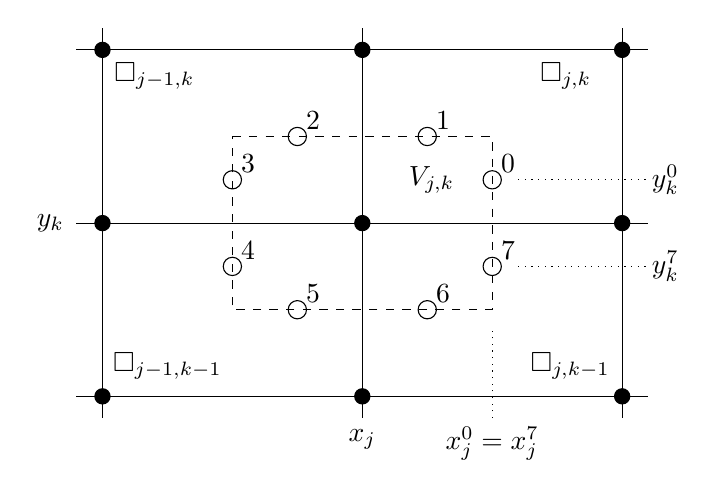
\begin{tikzpicture}[scale=1.1]
  %uncomment to see grid on which it was generated:
  %\draw[dotted,step=1.0,black,very thin] (0,0) grid (6,4);

  % strong grid around elements
  \draw (-0.3,0) -- (6.3,0);
  \draw (-0.3,2) -- (6.3,2);
  \draw (-0.3,4) -- (6.3,4);
  \draw (0,-0.25) -- (0,4.25);
  \draw (3,-0.25) -- (3,4.25);
  \draw (6,-0.25) -- (6,4.25);

  % nodes
  \filldraw (0,0) circle (2.5pt);
  \filldraw (3,0) circle (2.5pt);
  \filldraw (6,0) circle (2.5pt);
  \filldraw (0,2) circle (2.5pt);
  \filldraw (3,2) circle (2.5pt);
  \filldraw (6,2) circle (2.5pt);
  \filldraw (0,4) circle (2.5pt);
  \filldraw (3,4) circle (2.5pt);
  \filldraw (6,4) circle (2.5pt);

  % outline control volume
  \draw[dashed] (1.5,3) -- (4.5,3) -- (4.5,1) -- (1.5,1) -- cycle;

  % mark quadrature points

  \draw (4.5,2.5) circle (3.0pt) node[shift={(0.2,0.2)}] {0};
  \draw (3.75,3)  circle (3.0pt) node[shift={(0.2,0.2)}] {1};
  \draw (2.25,3)  circle (3.0pt) node[shift={(0.2,0.2)}] {2};
  \draw (1.5,2.5) circle (3.0pt) node[shift={(0.2,0.2)}] {3};
  \draw (1.5,1.5) circle (3.0pt) node[shift={(0.2,0.2)}] {4};
  \draw (2.25,1)  circle (3.0pt) node[shift={(0.2,0.2)}] {5};
  \draw (3.75,1)  circle (3.0pt) node[shift={(0.2,0.2)}] {6};
  \draw (4.5,1.5) circle (3.0pt) node[shift={(0.2,0.2)}] {7};

  % label elements and control volume
  \draw (3.8,2.5) node {$V_{j,k}$};
  \draw (5.35,3.7) node {$\square_{j,k}$};
  \draw (5.4,0.35) node {$\square_{j,k-1}$};
  \draw (0.6,3.7) node {$\square_{j-1,k}$};
  \draw (0.75,0.35) node {$\square_{j-1,k-1}$};

  % label center point
  \draw (3,-0.5) node {$x_j$};
  \draw (-0.6,2) node {$y_k$};

  % indicate coordinates of quadrature points
  \draw[dotted] (4.5,-0.25) -- (4.5, 0.8);
  \draw (4.5,-0.55) node {$x_j^0=x_j^7$};
  \draw[dotted] (4.8,2.5) -- (6.3, 2.5);
  \draw (6.5,2.5) node {$y_k^0$};
  \draw[dotted] (4.8,1.5) -- (6.3, 1.5);
  \draw (6.5,1.5) node {$y_k^7$};

\end{tikzpicture}

\end{center}
\caption{For equation \eqref{eq:siamstar} we evaluate $\bq^h(x,y)$ at eight quadrature points (numbered circles) along $\partial V_{j,k}$ (dashed).}
\label{fig:improvequadrature}
\end{figure}

The number of flux-evaluations for the improved method is twice that for the classical method, but the stencils are the same because the algebraic equation for the point $(x_j,y_k)$ uses the same nine nodal values of $H^h$.  (In fact both the improved and classical methods evaluate $\bq^h(x,y)$ at only four locations \emph{in each element}, the former at the midpoint of every side of every element.)

Eight half-edges make up $\partial V_{j,k}$, with each half-edge inside an element.  Thus one could propose further-improved quadrature, replacing the midpoint rule by higher-order methods (e.g.~2-point Gauss-Legendre).  Also, the $Q^1$ elements here could be replaced by higher-order $Q^2$ elements.  Though such methods have not been tested, even in the flat bed case the largest numerical SIA errors occur near the free boundary (margin) where the exact solution $H$ has low regularity \citep{Bueleretal2005}.  Thus higher-order quadrature and interpolation degree will probably not give much advantage.  Our improved method represents a measurable accuracy and Newton-method-convergence improvement over the classical Mahaffy method---see Results section---primarily because the improved method evaluates the flux approximation $\bq^h$ at points of continuity, not because the order of quadrature or interpolation is flawed in the classical scheme.

\cite{JaroschSchoofAnslow2013} show that the Mahaffy scheme can suffer from significant mass conservation errors at locations of abrupt change in the bed elevation.  In such cases, wherein the bed gradient dominates the thickness gradient, the mass conservation equation has ``hyperbolic'' character.  They implement a high-resolution upwind scheme \citep{LeVeque2002} based on flux form \eqref{eq:siafluxjsa}.  They show reduced mass conservation errors in the sense of giving numerical solutions which are closer in volume to an exact solution.  Their scheme expands the stencil, with equation \eqref{eq:siasteadyfd} at point $(x_j,y_k)$ involving thickness $H_{j+2,k}$, two cells away.  Note they solve the time-dependent problem, using explicit time-stepping.

By comparison, we now propose a minimal amount of first-order upwinding based on form \eqref{eq:fluxform} of the flux, but we do use their bedrock-step exact solution for accuracy-testing our implicit scheme.  Note that upwinding is not required for linear stability or non-oscillation of an implicit scheme, in the senses that apply to an explicit scheme \citep{MortonMayers2005}.  In \eqref{eq:fluxform} we denote the transport part by $\tilde \bq = \bW H^{n+2}$, where $\bW$ is computed by formula \eqref{eq:siaWdefine}.  So far we have evaluated the whole flux $\bq$ at each quadrature point, but to upwind we change the location where $H^{n+2}$ is evaluated according to the direction of $\bW$; evaluation of $D\grad H$ and $\bW$ at quadrature points is unchanged.

To be specific, let $0\le \lambda \le 1$.  Our upwind modification at $(x_j^0,y_k^0)$ uses the sign of
\begin{equation}
W^x_* = W^x(x_j^0,y_k^0),
\end{equation}
where $\bW=(W^x,W^y)$.  Note that the sign of $W_x^*$ is opposite that of the $x$-component of the bed gradient.  We shift the evaluation of $H$ in $\tilde \bq$ upwind by a quarter of an element width:
\begin{align}
&\tilde \bq^x(x_j^0,y_k^0)  \label{eq:upwindschemex} \\
&\quad = W^x_* \begin{cases}
                 H(x_j-\lambda \tfrac{\Delta x}{2},y_k^0)^{n+2}, & W^x_* \ge 0, \\
                 H(x_j+\lambda \tfrac{\Delta x}{2},y_k^0)^{n+2}, & W^x_* < 0.
             \end{cases} \notag
\end{align}
Noting that $\lambda=0$ corresponds to no upwinding and $\lambda=1$ is the maximum amount of upwinding that does not expand the stencil, after experimentation we chose $\lambda=1/4$; see Figure \ref{fig:upwindterm}.  This value of $\lambda$ is seen to be large enough to improve the convergence of the Newton solver but also to be small enough to generate substantial improvements in solution accuracy in the bedrock-step exact solution (Results section).  Upwinding at the other seven points along $\partial V_{j,k}$ (Figure \ref{fig:improvequadrature}) is achieved by similar formulas.

\begin{figure}[ht]
\begin{center}
\begin{tikzpicture}[scale=1.8]
  %uncomment to see grid on which it was generated:
  %\draw[dotted,step=1.0,black,very thin] (0,0) grid (6,4);

  % strong grid around elements
  \draw (-0.3,0) -- (3.3,0);
  \draw (-0.3,2) -- (3.3,2);
  \draw (0,-0.3) -- (0,2.3);
  \draw (3,-0.3) -- (3,2.3);

  % nodes
  \filldraw (0,0) circle (1.5pt);
  \filldraw (3,0) circle (1.5pt);
  \filldraw (0,2) circle (1.5pt);
  \filldraw (3,2) circle (1.5pt);

  % outline control volume
  \draw[dashed, thick] (-0.25,1) -- (1.5,1) -- (1.5,-0.25);

  % mark quadrature points
  \draw (1.5,0.5)  circle (2.0pt);
  \draw (0.75,1.0) circle (2.0pt);

  % mark upwind points
  \draw (1.125,0.5) node {$+$};
  \draw (1.875,0.5) node {$+$};
  \draw (0.75,0.75) node {$+$};
  \draw (0.75,1.25) node {$+$};

  % arrows to suggest upwinding
  %\draw[-latex] (1.6,0.4) -- (1.80,0.4);
  %\draw[-latex] (1.4,0.4) -- (1.20,0.4);
  %\draw[-latex] (0.65,1.05) -- (0.65,1.2);
  %\draw[-latex] (0.65,0.95) -- (0.65,0.8);

  % label elements and control volume
  \draw (2.7,1.7) node {$\square_{j,k}$};

  % label lower-left corner
  \draw (0,-0.5) node {$x_j$};
  \draw (-0.5,0) node {$y_k$};

  % indicate coordinates of quadrature point
  \draw (1.5,-0.5) node {$x_j^0$};
  \draw[dotted] (2.8,0.5) -- (3.2, 0.5);
  \draw (3.4,0.52) node {$y_k^0$};

\end{tikzpicture}

\end{center}
\caption{On element $\square_{j,k}$, when computing the flux at quadrature points (circles), upwinding of the flux term $\tilde \bq = \bW H^{n+2}$ evaluates the thicknesses $H$ at locations shown with ``$+$'', which are $\lambda=1/4$ of the way to the element boundary, according to the sign of a component of $\bW$.}
\label{fig:upwindterm}
\end{figure}

This form of upwinding does not expand the stencil.  It is most important at locations of low regularity of the solution.  We will see in verification (Results section) that it achieves higher solution accuracy than either the apparently second-order Mahaffy scheme or the reported results for the higher-resolution explicit scheme of \citep{JaroschSchoofAnslow2013}.

We call the method which combines both improve-ments---i.e.~more quadrature points and a bit of upwinding---the ``\Mstar'' scheme.  The convergence of the Newton method for solving the equations from this scheme is greatly improved in both verification cases and for real ice sheet geometries, compared to the classical Mahaffy scheme (Results section).


\section{Solution of the equations} \label{sec:solution}

We are ready to write down a system of nonlinear algebraic equations, so it remains to describe its numerical solution.  This is nontrivial because locating the free boundary (ice sheet margin) is an integral part of the problem of solving for steady state.  In fact, inequality constraints apply to each unknown.

Each equation in the \Mstar scheme is simply \eqref{eq:siamstar} with an upwind modification like \eqref{eq:upwindschemex} at the quadrature points.  The resulting highly-nonlinear system of $N=N_x N_y$ equations
\begin{equation}
F_{j,k}(\bH) = 0   \label{eq:nonlinsystem}
\end{equation}
determines $N$ unknowns, a vector $\bH=\{H_{j,k}\}$.  (Note ``$H^h(x,y)$'' and ``$\bH$'' are actually two notations for the same discrete thickness representation.)  System \eqref{eq:nonlinsystem} is not adequate by itself because each unknown thickness $H_{j,k}$ must be nonnegative,
\begin{equation}
\bH \ge 0.  \label{eq:nonlinconstraints}
\end{equation}

Requirements \eqref{eq:nonlinsystem} and \eqref{eq:nonlinconstraints} can be combined into a variational inequality \citep{JouvetBueler2012,KinderlehrerStampacchia1980}.  Equivalently, we can write them as a complementarity problem \citep{BensonMunson2006}:
\begin{equation}
\bH \ge 0, \quad \bF(\bH) \ge 0, \quad \bH \cdot \bF(\bH) = 0.  \label{eq:nonlincomplementarity}
\end{equation}
We solve \eqref{eq:nonlincomplementarity} by a ``constrained'' Newton solver, specifically by either the semi-smooth or the reduced-set method \citep{BensonMunson2006} implemented in PETSc \citep{Balayetal2014}.  Our open-source C code\footnote{Clone the repository at \texttt{https://github.com/bueler/sia-fve} and then see \texttt{README.md} in directory \texttt{petsc/} to compile \texttt{mahaffy.c} and run the examples.  The residual-evaluating method in \texttt{mahaffy.c} is called \texttt{FormFunctionLocal()}.} is brief as it contains just residual and Jacobian (below) evaluation subroutines.  Parallel grid management, Newton solver, iterative linear solver, and linear preconditioning jobs are all consigned to PETSc.  The choice of linear solver and preconditioner is made only at runtime.  Both multigrid \citep{Briggsetal2000} and additive-Schwarz-type domain decomposition \citep{Smithetal1996} preconditioning is found to allow convergence, but the latter is more robust.

The Jacobian of system \eqref{eq:nonlinsystem}, i.e.~the $N\times N$ matrix
\begin{equation}
J = \left(\,\frac{\partial F_{j,k}}{\partial H_{p,q}}\,\right), \label{eq:nonlinjacobian}
\end{equation}
can be computed via hand-calculated derivatives.  This additional effort (Appendix B) gives a speed-up by a rough factor of 1.5 over the alternative, namely finite-difference (FD) computation of Jacobian entries coming from additional residual (i.e.~$F$) evaluations.  Such FD Jacobians are efficiently-implemented in PETSc using ``coloring'' of the nodes \citep{CurtisPowellReid1974} so that, because of the nine-point stencil, only ten residual evaluations are needed to approximate $J$.  Because the grid is logically periodic and the stencil is three-by-three, however, the FD/coloring method requires grid dimensions $N_x$ and $N_y$ to each be divisible by three.

The standard theory of convergence of Newton's method shows that quadratic convergence should occur if $J$ is Lipshitz-continuous as a function of the unknowns \citep[and references therein]{Kelley2003}.  However, the flux $\bq$ is generally not smooth as a function of $\grad H$.  In particular, for $1<n<3$ the flux has a second derivative which is not Lipshitz-continuous with respect to changes in $\grad H$.  Because our Jacobian is the derivative of equations \eqref{eq:siamstar}, which already involves differentiating $\bq$ (in the limit where the control volume shrinks to zero), the behavior of second derivatives of $\bq$ determines the convergence of the solver.  Nonsmoothness of the flux is easiest to see in one dimension where equation \eqref{eq:siaflux} is
\begin{equation}
q(H,H') = - \Gamma H^{n+2} \left|H'+b'\right|^{n-1} (H'+b'). \label{eq:flux1d}
\end{equation}
When $n>1$,
\begin{equation}
\frac{\partial^2 q}{\partial H'^2} = - C H^{n+2} \left|H'+b'\right|^{n-3} (H'+b') \label{eq:ddflux1d}
\end{equation}
for $C>0$.  When $n=2$, for example, this function undergoes a step at $H'=-b'$, and thus is not Lipshitz.  When $1< n < 2$ the second derivative \eqref{eq:ddflux1d} is discontinuous and unbounded.  For $2<n<3$ it is continuous but with unbounded derivative.  Thus \eqref{eq:ddflux1d} is not Lipshitz-continuous for $1<n<3$.

Because we want methods that work for all exponents $n\ge 1$, we regularize by replacing
\begin{equation}
|\grad s| \to \left(|\grad s|^2 + \delta^2\right)^{1/2}, \label{eq:nonlinregularization}
\end{equation}
with $\delta = 10^{-4}$, from now on when we compute the flux $\bq$ and its derivatives.  This regularization, which makes little difference when the surface slope is of order $10^{-3}$ or larger, is not surprising because it is similar to that used in regularizing the viscosity in the Stokes equations \citep{GreveBlatter2009}, and other distributed stress balance models \citep[for example]{BrownSmithAhmadia2013,BuelerBrown2009}.

A Newton solver requires an initial iterate $H^{(0)}$.  We generate it by a heuristic which seems to work adequately-well for both ice sheet- and glacier-scale problems, and which is suggested by \cite{JouvetGraeser2013} in a time-stepping context.  From the steady surface mass balance data $m_{j,k}$, in meters per year, we compute
\begin{equation}
H_{j,k}^{(0)} = \max\left\{0,1000\,m_{j,k}\right\}  \label{eq:nonlininitialheuristic}
\end{equation}
In other words, we build the initial ice sheet thickness simply by piling up one thousand years of accumulation, without flow.

Additionally we apply a simple ``parameter continuation'' scheme, to aid in the convergence of the Newton iteration on our degenerate, nonlinear free-boundary problem.  We first apply the Newton method to an easier free-boundary problem, one with constant diffusivity.  Then we adjust a continuation parameter $\eps$ until we are solving the full SIA free-boundary problem.  Specifically, for $0 \le \eps \le 1$ we define
\begin{equation}
n(\eps) = (1\!-\eps) n + \eps n_0 \text{ and } D(\eps) = (1\!-\eps) D + \eps D_0  \label{eq:continuationND}
\end{equation}
where $n$ is the original exponent, $D$ is computed in \eqref{eq:siaflux}, $n_0=1$, and $D_0$ is a typical scale of diffusivities for the problem (e.g.~$D_0=0.01$ $\text{m}^2\,\text{s}^{-1}$ for a glacier problem or $D_0=10$ $\text{m}^2\,\text{s}^{-1}$ for an ice sheet).  Note $n(1)=n_0$ and $D(1)=D_0$ while $n(0)=n$ and $D(0)=D$.  We then consecutively solve free-boundary problems corresponding to thirteen values of $\eps$:
\begin{equation}
\eps_i = \begin{cases}
           (0.1)^{i/3}, & \text{for } i=0,\dots,11, \\
           0, & i=12,
         \end{cases}  \label{eq:continuationseq}
\end{equation}
so that, until the last stage $\eps_{12}=0$, the parameter $\eps_i$ is reduce by an order of magnitude as $i$ increases by three.

We start with $\eps_0=1$ so we are solving \eqref{eq:nonlincomplementarity} with values $n=n_0$ and $D=D_0$ from \eqref{eq:continuationND}, and initial iterate $H^{(0)}$ from \eqref{eq:nonlininitialheuristic}.  Once the Newton solver for this problem converges, we take the solution as the initial iterate for problem \eqref{eq:nonlincomplementarity} but using the second value $\eps_1=(0.1)^{1/3}\approx 0.46$ in \eqref{eq:continuationND}.  Continuing in this way we eventually solve the unregularized $n(0)=n$ and $D(0)=D$ problem.  The first twelve stages $\eps_0,\dots,\eps_{11}$ generate a very high-quality initial iterate for the un-modified SIA calculation ($\eps_{12}=0$).

The first $\eps_0=1$ problem is a Laplacian obstacle problem \citep{KinderlehrerStampacchia1980}, namely $-\Div(D_0 \grad s) = m$ subject to the constraint $s\ge b$.  Starting with this well-behaved free-boundary problem, which nonetheless uses all the data $b,m$, allows the Newton solver to generate a first estimate of the ice-covered domain.  In particular, at the end of the first stage the ice margin has moved from the equilibrium line (i.e.~because of initial iterate \eqref{eq:nonlininitialheuristic}) into the ablation zone as expected.

The relationship between our steady-state computations and fully-implicit time-stepping methods for equation \eqref{eq:siaevolution} deserves examination.  We can exploit the relationship to make the Newton solver highly-robust for real-data cases.

Observe that by solving for steady state we effectively take infinite-duration implicit time steps in the time-dependent problem.  Indeed, the backward-Euler \citep{MortonMayers2005} approximation of equation \eqref{eq:siaevolution} is
\begin{equation}
\frac{H^\ell - H^{\ell-1}}{\Delta t} + \Div \bq^\ell = m \label{eq:backwardeuler}
\end{equation}
where $H^\ell(x,y) \approx H(t_\ell,x,y)$ is the unknown thickness, $H^{\ell-1}$ is known from the previous time-step, and $\bq^\ell$ is the flux computed from \eqref{eq:siaflux} using $H^\ell$.  Our method extends easily from solving \eqref{eq:nonlincomplementarity} to solving a single time-step of \eqref{eq:backwardeuler}, subject as before to the constraint $\bH\ge 0$.  For finite $\Delta t$, problem \eqref{eq:backwardeuler} is practically easier because the initial iterate can be taken to be the initial value, or the solution at the previous time step, and because the continuation sequence can be avoided or truncated to only include the smallest $\eps$ value.  More important than that, however, is the key fact is that solving \eqref{eq:backwardeuler} gets easier as $\Delta t\to 0$, essentially because the Jacobian $J$ has a more-positive diagonal due to the $H^\ell/\Delta t$ term in \eqref{eq:backwardeuler}.  If a Newton iteration fails to converge in the steady-state case, we might hope that the same scheme would still solve \eqref{eq:backwardeuler} successfully for finite $\Delta t$, and this is precisely what we see in practice.  Switching from the steady state problem to long (e.g.~100 year) backward-Euler time steps is a ``recovery strategy'' for dealing with Newton solver difficulties when dealing with highly-irregular bed topography data in the steady state problem (Results section).


\section{Results}

In this section we first apply our method in two examples, with and without flat beds, where exact solutions are known.  On the one hand our method uses the \Mstar scheme \eqref{eq:siamstar} to generate discrete system \eqref{eq:nonlincomplementarity}, so we compare its performance to the classical Mahaffy scheme.  We use the exact solutions to evaluate the convergence of the discrete solution to the continuum solution under grid refinement (verification).  On the other hand, our method has a regularization \eqref{eq:nonlinregularization}, a continuation scheme \eqref{eq:continuationND}, and a constraint-adapted Newton solver from PETSc to solve the system, and so we also evaluate the convergence of the Newton iteration in an exact solution case.  After that we apply the method in an extended Greenland ice sheet example using high-resolution bedrock topography.  All computations in this section are in two horizontal variables, but we show verification case results along flow lines starting from the center of the ice sheet or glacier.

\subsection{Verification cases}

An angularly-symmetric steady-state exact solution \citep{Bueler2003} exists in the flat bed case; see also subsection 5.3 of \cite{vanderVeen2013}.  This ``dome'' exact solution, with parameters suitable for a medium-sized ice sheet, is shown in Figure \ref{fig:domeprofile}.  The numerical results from our \Mstar method are very close to the exact solution, with only an error at the last positive-thickness grid point barely-visible.  However, results for 25 km and 12.5 km grids are compared in the inset to illustrate the consequences of unbounded gradient at the margin.  Namely, there are relatively-large thickness errors which decay slowly under grid refinement \citep{Bueleretal2005}.

\begin{figure}[ht]
\onecol{domeprofile.pdf}
\caption{Result from \Mstar method on a $\Delta x=\Delta y=25$ km grid (dots) compared to the dome exact solution.  The detail of the margin adds results from a 12.5 km grid  (diamonds).}
\label{fig:domeprofile}
\end{figure}

On this exact solution we can measure the maximum and average thickness errors from both classical Mahaffy and \Mstar methods.  As shown in Figure \ref{fig:domeverif}, both methods show very slow convergence of maximum error, for the reason we have just stated.  The decay of the average error for \Mstar, which reduces to about 1 m for the three finest grids, is distinctly-better than for classical Mahaffy.  However, because of unbounded gradient at the margin, the \Mstar decay rate of $O(\Delta x^{1.47})$ is less good than the $O(\Delta x^2)$ convergence rate expected from both methods.  In fact, as indicated in the figure by gray circles, the Newton method fails to converge for all classical Mahaffy runs except the coarsest.  This improved convergence of the \Mstar scheme, which only differs from the classical one by improved quadrature in this flat bed case, is seen in all cases tried.  Though the \Mstar method fails to converge on the two finest grids, at the $\eps_{12}=0$ level of the continuation sequence only, these cases fully-converge if the problem is changed to a backward Euler step \eqref{eq:backwardeuler} of duration $100.0$ years (not shown).

\begin{figure}[ht]
\onecol{domeverif.pdf}
\caption{Average and maximum error under grid refinement using the dome exact solution, for the \Mstar (stars) and classical Mahaffy (squares) methods.  Gray circles indicate runs where the Newton method diverged before the last $\eps_{12}=0$ stage of continuation sequence \eqref{eq:continuationseq}.}
\label{fig:domeverif}
\end{figure}

Figure \ref{fig:newtonconv} shows clear evidence of quadratic, or at least superlinear, convergence from the Newton solver, in runs where the relative tolerance (i.e.~residual 2-norm reduction factor) is $10^{-10}$.  At each stage $\eps_i$ of the continuation scheme, the computed residual shows the characteristic curved drop, on log-residual-norm versus iteration number axes, associate to a successful Newton solve \citep{Kelley2003}.  As is typical of Newton solvers, either this sudden drop of residual norm is observed or divergence occurs.

\begin{figure}[ht]
\onecol{newtonconv.pdf}
\caption{Residual norm versus iteration number for each continuation stage.  The SIA problem itself is the last $\eps_{12}=0$ curve.}
\label{fig:newtonconv}
\end{figure}

To test performance on non-flat and non-smooth beds, we use a glacier-scale bedrock-step exact solution by \cite{JaroschSchoofAnslow2013}.  As shown in Figure \ref{fig:bedstepprofiles}, the exact thickness is discontinuous at the cliff, because the thickness goes to zero on the uphill side and has a nonzero value on the downhill side.  (The computation uses two horizontal dimensions but is constant and periodic in the $y$-direction.)  The Figure also shows results from \Mstar versions without upwinding (i.e.~$\lambda=0$ in formula \eqref{eq:upwindschemex}; ``\Mstarnoup'') and using the maximum upwind that does not expand the stencil ($\lambda=1$; ``\Mstarfullup'').  These results explain why we have chosen $\lambda=1/4$.  For \Mstarnoup there are very large errors on the downhill side of the cliff, though the uphill side is fine \citep{JaroschSchoofAnslow2013}.  For \Mstarfullup the downhill side is fine but now the uphill thickness is much too large.  Just a bit of upwinding---$\lambda=1/4$ works but other values would too---captures the flux at the cliff so that both uphill and downhill thicknesses are good.

\begin{figure}[ht]
\onecol{bedstepprofiles.pdf}
\caption{Results from \Mstar method, and it upwinding variations, compared to the bedrock-step exact solution ($\Delta x=1000$ m).}
\label{fig:bedstepprofiles}
\end{figure}

To compare to results in \citep{JaroschSchoofAnslow2013}, we applied the \Mstar method on grids with $\Delta x=\Delta y = 1000,500,250,125$ m.  When we measure maximum thickness errors, there is \emph{no} evidence of convergence as the grid is refined, and for average thickness errors the evidence of convergence is unconvincing (not shown), but these norms are not reported by \cite{JaroschSchoofAnslow2013}, so we cannot compare.  Maximum errors are not, however, expected to decay because even an interpolant of the discontinuous exact solution will not exhibit maximum norm convergence.  The theory of FE methods does not suggest convergence in average error either, because of the extremely-low regularity of the exact solution \citep{Elmanetal2005}.

However, like \cite{JaroschSchoofAnslow2013} we can examine relative volume error, a weak quality measure which is not a norm, in addition to the visual evidence.  Table \ref{tab:bedstepvol} shows the value
\begin{equation}
100\, \frac{V_{\text{numerical}} - V_{\text{exact}}}{V_{\text{exact}}}.
\end{equation}
The second, third, and fourth columns are from the same three versions of the \Mstar method shown in Figure \ref{fig:bedstepprofiles}.  Again we see why $\lambda=1/4$ is preferred to the upwinding alternatives.  The last two columns show the results reported by \cite{JaroschSchoofAnslow2013} for their best ``Superbee''-limited MUSCL scheme and for their implementation ``M2'' of the classical Mahaffy scheme.

\begin{table}[ht]
  \caption{Relative volume differences, as percentage, for results on the \cite{JaroschSchoofAnslow2013} bedrock-step exact solution.  ``\Mstar'' columns show three upwinding variations (see text).  ``NC'' indicates a Newton method convergence failure.  ``Superbee'' and ``M2'' are results from \cite{JaroschSchoofAnslow2013} (see text).}
  \vskip4mm \centering
  \begin{tabular}{lccccc}
    $\Delta x$ & \Mstar & \Mstarnoup & \Mstarfullup & Superbee & M2 \\  \hline
\input{bedsteptable.tex}
  \end{tabular}
  \label{tab:bedstepvol}
\end{table}

These good results from a little bit of first-order upwinding in our implicit \Mstar scheme have discouraged us from expensive further attempts to improve the advection scheme, until such time as new precise evidence is available.  Note \cite{JaroschSchoofAnslow2013} have explicit implementations, so the fact that implementations of the ``Superbee'' and other high-resolution flux methods have ``if-then'' conditionals \citep{LeVeque2002} is not dangerous.  For our implicit Newton solver, however, which needs a differentiable residual function to get a well-conditioned Jacobian, the additional non-smoothness of high-resolution flux methods suggests caution.  Our bit of upwinding seems helpful to Newton convergence, however.

%FIXME: idea. upwinding in steady-state case is ``adding off-diagonal temr to nonsymmetric matrix so as to help invertibility''

\subsection{Greenland}

FIXME: add whole Greenland model; compute \Mstar SIA solution with present-day climate in one step on fairly high res (1km); like \cite{JouvetBueler2012} result but much higher res and replacing fixed-point iteration by continuation 

\begin{figure}[ht]
\onecol{grnrobusteps.pdf}
\caption{Lowest value of $\eps_i$ in the continuation scheme where the Newton method converges on the steady-state problem.}
\label{fig:grnrobusteps}
\end{figure}

\section{Discussion and Conclusion} \label{sec:conclusion}

FIXME: The first idea in the paper is that a FVE interpretation is compatible with the original Mahaffy FD scheme.  The second idea is that the classical method's flux approximation is discontinuous along element edges.  We improve the method by doubling the number of quadrature points.  For nonflat beds we also add a bit of upwinding, and tests show the effectiveness.  The new \Mstar method is more accurate and its Newton iterations converge better, than the classical scheme.  We have applied the method at large scale and high resolution on real data, and it converges.  The computed examples using this method are novel, except for \cite{JouvetBueler2012}, by going directly to steady state from zero ice.

FIXME: We have been basically flux-agnostic.  The same basic FVE works as long as there is a way of computing $\bq^h(x_j^s,y_k^s)$ from the current $\bH$.  Thus our methods can be extended to include sliding and flow models based on membrane stress balances. 

\section*{Acknowledgements}
This work was supported by NASA grant \#NNX13AM16G and a grant of high-performance computing resources from the Arctic Region Supercomputing Center.


%         References
\bibliography{siafve}
\bibliographystyle{igs}

\appendix
\section{Appendix A.  Unstructured FVE scheme}  \label{sec:appA}

FIXME: the same \Mstar idea can be extended to dual Delaunay/Voronoi meshes (e.g.~the meshes from \cite{EgholmNielsen2010,Ringleretal2013}) using $P^1$ elements on the Delaunay triangulation, and doing quadrature on the Voronoi-cell edges by splitting these edges where the element (i.e.~triangle) boundaries cross (perpendicularly) the Voronoi-cell edges.  This improves on the \cite{EgholmNielsen2010} method by exploiting an underlying $P^1$ element approximation to approximate the flux, instead of using the moving least squares method.

\begin{comment}
Here is what the MPAS Land-Ice User's Manual version 3.0 says:
\begin{quote}
\small
Velocities and fluxes are calculated on the midpoint of Voronoi cell edges.  The normal component of surface slope is calculated on cell edges using surface elevation at adjacent cell centers.  The tangential component of surface slope is calculated on cell edges using surface elevation at adjacent vertices. The surface elevation at vertices is calculated from the values at adjacent cell centers using barycentric interpolation. Ice thickness on edges is calculated as the average of the adjacent cell center values (2nd-order approximation).
\end{quote}
Looking at this, and their code, I don't think they think of it as Petrov-Galerkin
\end{comment}

\section{Appendix B. Jacobian computation}  \label{sec:appB}

Though finite differencing can be used to approximate the Jacobian \eqref{eq:nonlinjacobian} of the nonlinear algebraic system \eqref{eq:nonlinsystem}, convergence of the Newton iteration is accelerated by analytical evaluation.  To sketch the calculation of the Jacobian for the \Mstar method, we recall that each equation $F_{j,k}(\bH)=0$ in the system comes from equation \eqref{eq:siamstar},
\begin{equation}
  F_{j,k} = \sum_{s=0}^7 \bc_s\cdot \bq^h(x_j^s,y_k^s) - m_{j,k}\,\Delta x\,\Delta y.  \label{eq:res}
\end{equation}
As the stencil of the \Mstar scheme is the nine-node box shown in Figure \ref{fig:fdfemgrids}b, each row of the Jacobian, corresponding to location $j,k$ in the grid, has nine nonzero entries, corresponding to locations $p,q$ where $F_{j,k}$ depends on $H_{p,q}$, and thus where $\partial F_{j,k}/\partial H_{p,q}$ is nonzero.  We compute
\begin{equation}
\frac{\partial F_{j,k}}{\partial H_{p,q}} = \sum_{s=0}^7 \bc_s\cdot \frac{\partial \bq^h(x_j^s,y_k^s)}{\partial H_{p,q}}. \label{eq:jacQsum}
\end{equation}
In fact $\partial \bq^h(x_j^s,y_k^s)/\partial H_{p,q}$ is nonzero only if $H_{p,q}$ is one of the four nodal values on the element $\square_{u,v}$ containing the quadrature point $(x_j^s,y_k^s)$.  Recalling that we index the four corners of $\square_{u,v}$ by $\ell=0,1,2,3$---see Figure \ref{fig:fdfemgrids}b---we need to write code to compute
\begin{equation}
\bQ_\ell^s = \frac{\partial \bq^h(x_j^s,y_k^s)}{\partial H_\ell} \label{eq:jacthegoal}
\end{equation}
when $(x_j^s,y_k^s)$ is in $\square_{u,v}$.

Having made the goal clear, we recall the quantities which are easiest to compute in a $Q^1$ FE method.  If $\xi=(x-x_u)/\Delta x$ and $\eta=(y-y_v)/\Delta y$ are local coordinates on $\square_{u,v}$, so that $0\le \xi,\eta \le 1$, then bilinear interpolation defines a function $H_{u,v}=H_{u,v}(\xi,\eta)$ on $\square_{u,v}$ from interpolation of the four nodal values $H_\ell$---see the bilinear basis functions in equation \eqref{eq:elementbasis}.  The bed elevation function $b_{u,v}$ is similarly defined.

Differentiation with respect to $\xi$ and $\eta$ gives vector-valued function $(\grad H)_{u,v}$ and $(\grad b)_{u,v}$.  Differentiation with respect to $H_\ell$ gives the scalar function $\partial H_{u,v}/\partial H_\ell$ and the vector-valued function $\partial (\grad H)_{u,v}/\partial H_\ell$.  We write code for each of these functions, which use local coordinates $\xi,\eta$ on $\square_{u,v}$.

Now recall $D$ is defined in \eqref{eq:siafluxdiffusion} and $\bW$ is defined in \eqref{eq:siaWdefine}.  Therefore we next write code to compute element-wise function $D_{u,v}$, $\partial D_{u,v}/\partial H_\ell$, $\bW_{u,v}$, and $\partial \bW_{u,v}/\partial H_\ell$, again all in local coordinates $\xi,\eta$ on $\square_{u,v}$.

\newcommand{\uppoint}{(\xi_{\text{up}}^s,\eta_{\text{up}}^s)}
Denote the local coordinates of the quadrature point $(x_j^s,y_k^s)$ on the element $\square_{u,v}$ by $\xi^s = (x_j^s-x_u)/\Delta x$ and $\eta^s = (y_k^s-y_v)/\Delta y$.  Note that for each quadrature point, as in Figure \ref{fig:upwindterm}, upwinding determines an additional evaluation point, whose local coordinates are denoted $\uppoint$.

In these terms, from \eqref{eq:fluxform}, for the evaluation of the residual, i.e.~\eqref{eq:res}, we write code to compute
\begin{align}
\bq^h(x_j^s,y_k^s) &= - D_{u,v}(\xi^s,\eta^s)\, (\grad H)_{u,v}(\xi^s,\eta^s) \label{eq:resfinalformula} \\
   &\quad + \bW_{u,v}(\xi^s,\eta^s) \, H_{u,v}\uppoint^{n+2}. \notag
\end{align}
For the evaluation of the Jacobian, i.e.~\eqref{eq:jacthegoal}, we write code to compute
\begin{align}
\bQ_\ell^s &= - \frac{\partial D_{u,v}}{\partial H_\ell}(\xi^s,\eta^s)\, (\grad H)_{u,v}(\xi^s,\eta^s) \label{eq:jacfinalformula} \\
   &\quad - D_{u,v}(\xi^s,\eta^s)\, \frac{\partial (\grad H)_{u,v}}{\partial H_\ell}(\xi^s,\eta^s) \notag \\
   &\quad + \frac{\partial \bW_{u,v}}{\partial H_\ell}(\xi^s,\eta^s) \, H_{u,v}\uppoint^{n+2} \notag \\
   &\quad + (n+2) \bW_{u,v}(\xi^s,\eta^s)\, H_{u,v}\uppoint^{n+1} \notag \\
   &\qquad\quad \cdot \frac{\partial (\grad H)_{u,v}}{\partial H_\ell}\uppoint. \notag
\end{align}



\end{document}
